\chapter{Analyse d'une des publicités}

\label{Analyse d'une des publicités}

\section{Présentation de la publicité analysée}

De ce contexte, né en 1964, de la plume de l'illustrateur New-Yorkais \textit{Haddon Sundblom}, la réclame qui nous intéresse.

\begin{figure}[th]
\centering
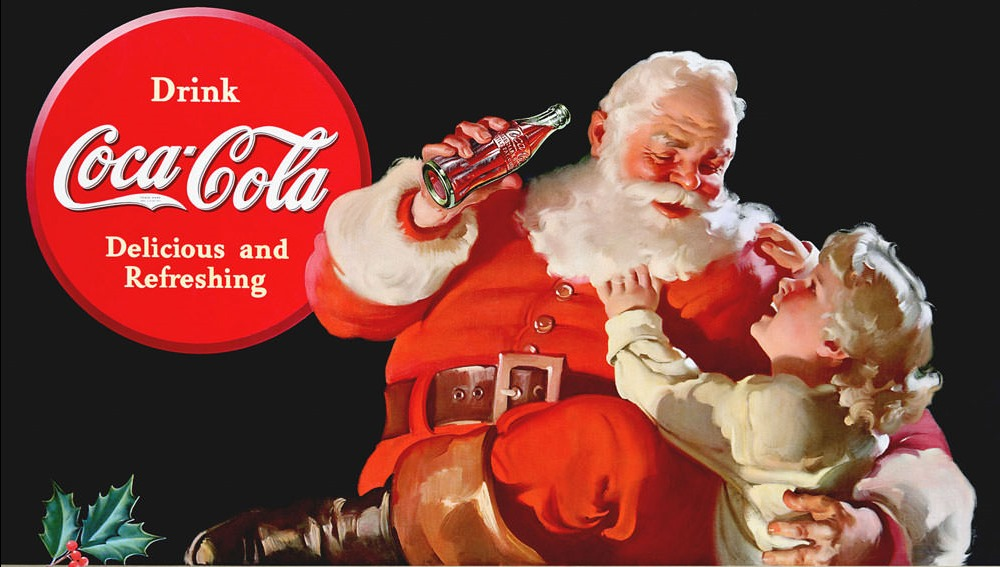
\includegraphics[width=130mm]{medias/affiche_coca}
\decoRule
\caption{Réclame étudiée dans cette dossier.}
\end{figure}

J'ai choisi cette publicité en particulier car elle résume en idées simples tous les messages que l'entreprise souhaitait faire passer pendant cette période de son histoire.

%----------------------------------------------------------------------------------------

\section{Analyse descriptive de la publicité}

\subsection{Une présentation sobre}

On voit tout d'abord qu'il n'y a aucun élément superflu, le fond est noir, ce qui nous fait comprendre que cette réclame veut uniquement montrer ce qu'elle a à dire, mettant d'avantage en avant ses propos.\\
Tout élément ici a donc son importance; À première vue, on remarque entre-autres, trois éléments principaux dans la composition: le père noël, ayant une place centrale quoique légèrement déportée par la droite afin de laisser place au logo coca-cola, dans un cercle rouge avec deux slogans (nous y reviendrons). On pourrait aller jusqu'à formaliser et penser que l'utilisation du cercle rouge n'est pas dû à un simple hasard mais bien au rappel des capsules de bouteilles en verre, renforçant d'avantage de façon non-consciente la marque dans nos esprits.

\subsection{Une présentation attrayante}

Le fond noir ne sert pas qu'à mettre en avant les éléments, mais fait même mieux ressortir les couleurs prédominantes de la marque. On remarque que tout est aussi fait pour associer le bonheur avec la boisson, en particulier avec le sourire des personnages.

\subsection{Un rappel des thèmes hivernaux}

J'ai délibérément omis de parler jusqu'à maintenant de quelques éléments-clef; Tout d'abord, le plus évident, la présence du père-noël, qui viendrait égayer avec du soda la vie des enfants en cette période. Cependant, un détail qui reste capital est la branche de gui verte en bas à gauche de la composition: celle-ci a plusieurs fonctions, notamment renforcer le thème de Noël via un élément que l'on retrouve à ce moment de l'année ainsi que de complémenter le rouge omniprésent de l'image avec un vert qui permet d'associer plus facilement les fêtes de fin d'année avec la marque via ce code couleur normalisé qu'est le rouge et le vert.

\subsection{Analyse colorimétrique}

\begin{figure}[th]
\centering

\includegraphics[width=130mm]{medias/palette}
\decoRule
\caption{Palette de couleurs de l'image}
\end{figure}

En analysant et en effectuant une moyenne des couleurs existantes, on voit là aussi que rien n'a été laissé au hasard.
Cette palette permet d'abord de corroborer mes précédents dires sur l'importance des couleurs et leurs significations;
\begin{itemize}
\item[\textcolor{palette1}{\textbullet}] Le \textbf{noir} sert simplement à donner un contraste et une importance aux autres couleurs;
\item[\textcolor{palette2}{\textbullet}] Le \textbf{rouge} rappelle principalement la marque et les couleurs festives. De plus, quand on se renseigne sur  la théorie des couleurs dans le marketing \parencite{Ref2}, le rouge est symbole de puissance et d'impulsivité;  Cette couleur est à l'image de la marque et à une sorte de fonction \textbf{conative}: elle est parfaite pour inciter le consommateur à acheter rapidement.
\item[\textcolor{palette3}{\textbullet}] Le \textbf{blanc lin} sert de d'opposition au noir, en plus d'être une couleur représentant généralement la pureté, raison pour laquelle la petite fille est habillé de cette couleur. En prime, on notera qu'en plus d'être la deuxième couleur de la marque (visible avec la police d'écriture par exemple), c'est aussi une des couleurs données par le dessinateur au "Santa-Claus";
\item[\textcolor{palette4}{\textbullet}] Le \textbf{vert} représente, comme vu dans la partie précédente, une des deux couleurs de Noël. Dans le domaine du marketing, on peut associer le vert à la sérénité ou à l'équilibre;
\item[\textcolor{palette5}{\textbullet}] En plus des précédentes couleurs, on en remarque une nouvelle qui nous n'avons pas forcément analysé mais qui constitue la base du produit: le \textbf{brun}. En effet, c'est la couleur principale de la boisson, et c'est celle qui est inscrite dans la scène de façon plus discrète afin de potentiellement influencer notre subconscient;
\end{itemize}

%----------------------------------------------------------------------------------------

\section{Le but et les moyens de la publicité}

\subsection{Audience-cible}

Cette publicité, et d'une façon plus générale, cette campagne, cibler de prime abord \textbf{les jeunes}, comme nous pouvons le voir sur l'image, mais ce n'est pas pour autant le seul groupe visé. En réalité, Coca-Cola essaye d'atteindre \textbf{le plus de monde possible} afin d'être les plus versatile du marché. Contrairement aux boissons alcoolisés par exemple, les sodas sont accessibles par tous: d'une certaine façon, cette publicité nous montre que si même le père noël, figure festive mythique, se permet de boire un soda, pourquoi-pas les gens qui sont sujets à cette réclame ?

\hfill \break

\begin{figure}[th]
\centering
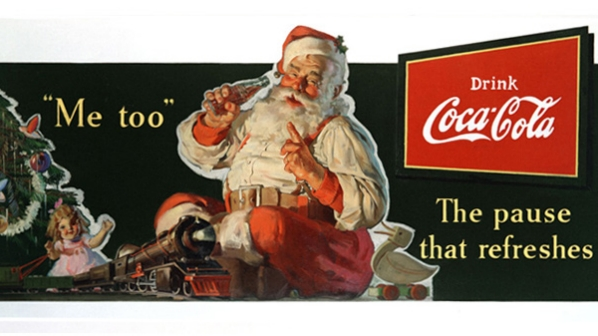
\includegraphics[width=140mm]{medias/meetoo}
\decoRule
\caption{"Moi aussi", autre réclame de la marque}
\end{figure}
\newpage

\subsection{"\textit{Drink Coke}"}

Il faut avant tout savoir quel est le but de cette opération; En effet, on peut grossièrement catégoriser les types de publicités en trois catégories, toutes aux ambitions bien différentes :

\renewcommand{\labelitemi}{$\ast$}
\begin{itemize}
\item La publicité argumentation : elle défend une idée et/ou tente de modifier l’opinion des récepteurs.
\item La publicité informative : elle a pour fonction de livrer au récepteur une information.
\item La publicité incitative : ce type de publicités poussent les gens à agir et à acheter un produit
\end{itemize}

On remarque que la stratégie commerciale qu'emploie Coca-Cola tient de l'ordre de \textbf{la publicité incitative}:
on le remarque tout d'abord dans ce qui était leur slogan que l'on retrouve sur cette publicité, "\textit{Drink Coca-Cola.}" ("\textit{Bois Coca-Cola.}"), qui ressemble fortement à une sorte \textbf{d'ordre} voire d'injonction que le consommateur reçoit. De plus, on remarque que cette méthode agressive transparaît aussi dans d'autres slogans, comme par exemple en 1952 avec "\textit{What you want is a Coke.}" ("\textit{Ce que vous avez besoin, c'est d'un Coca-Cola.}").

\begin{figure}[th]
\centering
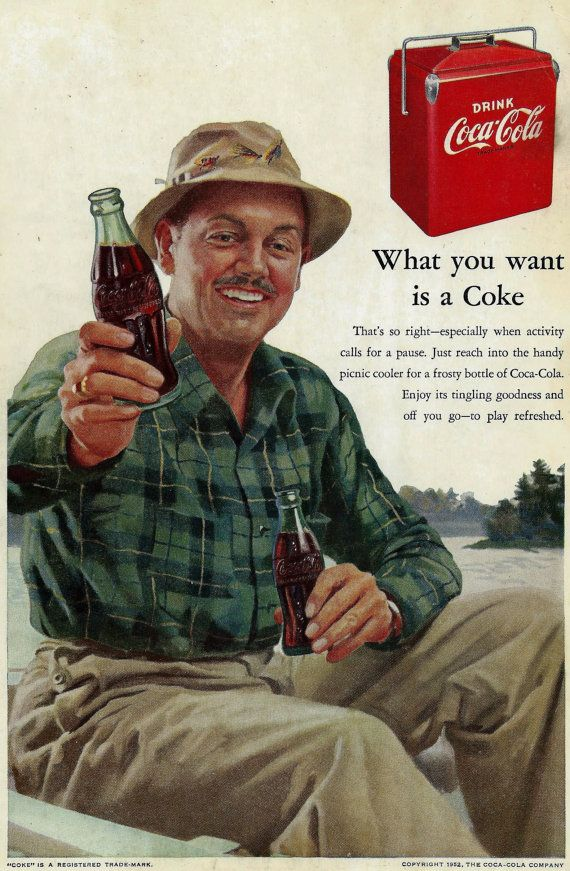
\includegraphics[width=80mm]{medias/poster_coca}
\decoRule
\caption{Exemple de réclame voulant forcer les envies des consommateurs }
\end{figure}
\newpage

\subsection{"\textit{Delicious \& Refreshing}"}

« Delicious \& Refreshing » (Délicieux et rafraîchissant), deux mots qui définissent les dites "qualités gustatives" du Coca‑Cola, deux mots qui sont en quelque sorte leur deuxième slogan apparaissant non seulement ici, mais aussi sur la quasi-totalité des publicités ou autres spots publicitaires.
Lancé en 1904, ce slogan met en avant les deux atouts du produit : \textbf{la promesse d'un goût unique et une sensation de fraîcheur}; ce slogan est personnifié généralement par un consommateur en action – comme par exemple ici avec le père-noël. Il s'agit là d'un principe que l’on retrouve régulièrement dans la communication de la marque, et il s'agit d'une pratique toujours d'actualité chez la marque.

\begin{figure}[th]
\centering
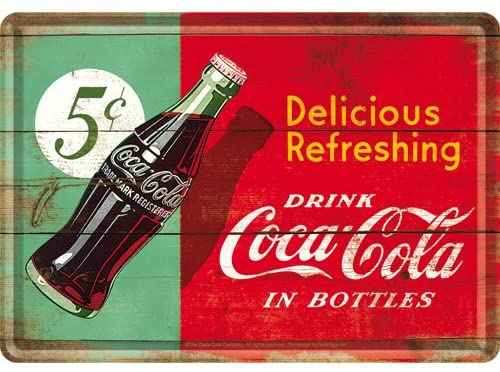
\includegraphics[width=80mm]{medias/panneau_coca}
\decoRule
\caption{Exemple de réclame voulant forcer les envies des consommateurs }
\end{figure}

\subsection{Miser sur le long-terme}

La superposition de l'apparition du père-noël avec le coca-cola crée une situation anormale qui attire l'attention. Ensuite, le nombre important de publicités reprenant les codes de cette dernière vont permettre à la compagnie d'associer Noël avec leur produit - Pari portant ses fruits car, en 2021, on retrouve encore ces mêmes éléments dans leurs campagnes \parencite{Ref3}.\\
\textbf{La récurrence est donc un des élément principal de la stratégie marketing de Coca-Cola}.

\subsection{Associer Coca à la "\textit{magie de noël}"}

Le but premier de ces illustrations est \textbf{l'association de la fête avec la boisson}, d'une part pour pouvoir continuer à faire profit même en période hivernale et d'autre part afin de faire en sorte de coupler une image déjà ancrée à la marque. On fait appel à la subjectivité du consommateur et on crée un lien affectif entre ce dernier et le produit via les fêtes afin de ne plus pouvoir dissocier les deux.

\subsection{Une exportation mondiale}

La marque à su réaliser un tour de force, non seulement avec donc la récurrence et avec son association, mais aussi avec \textbf{le contexte politico-économique}. Il faut se rappeler que cette période de réclames correspond à la seconde guerre-mondiale, et, à sa fin, un grand mouvement d'exportation de valeurs et de culture s'effectue avec plusieurs pays, c'est le cas de l'hexagone avec les chewing-gums et le fameux "père-noël Coca".\parencite{Ref4}

\begin{figure}[th]
\centering
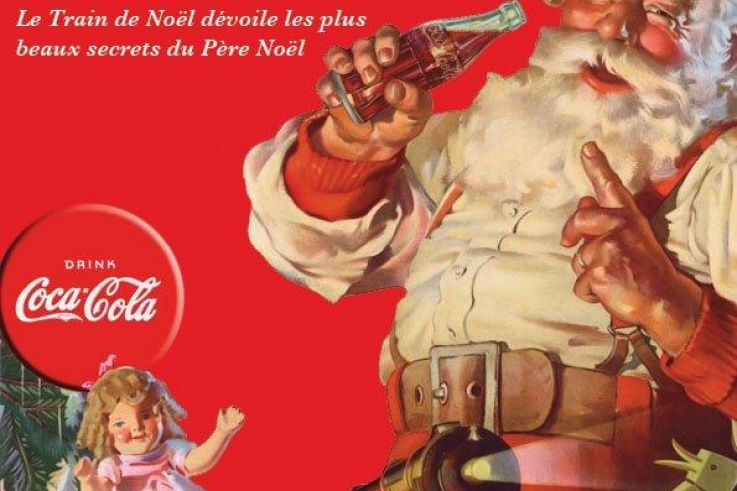
\includegraphics[width=110mm]{medias/france_coca}
\decoRule
\caption{Première apparition de la campagne en France}
\end{figure}
